\documentclass[12pt,letterpaper]{article}
\usepackage[left=1in,right=1in,top=1in,bottom=1in]{geometry}
\usepackage{amssymb}
\usepackage[fleqn]{amsmath}
\usepackage{amsthm}
\usepackage{graphicx}
\usepackage{listings}
\usepackage{courier}
\usepackage[usenames,dvipsnames]{color}    
\DeclareGraphicsExtensions{.png,.pdf}
\graphicspath{}

\title{The Influence of Receiver Routes and Separation from Defenders on Third Down Conversions}
\author{Lingge Li, Hua Xie, Micah Jackson, and Kyle Sneeden}

\linespread{1.2}

\lstset{
  language=R,                     % the language of the code
  basicstyle=\tiny\ttfamily, % the size of the fonts that are used for the code
  numbers=left,                   % where to put the line-numbers
  numberstyle=\tiny\color{Blue},  % the style that is used for the line-numbers
  stepnumber=1,                   % the step between two line-numbers. If it is 1, each line
                                  % will be numbered
  numbersep=5pt,                  % how far the line-numbers are from the code
  backgroundcolor=\color{white},  % choose the background color. You must add \usepackage{color}
  showspaces=false,               % show spaces adding particular underscores
  showstringspaces=false,         % underline spaces within strings
  showtabs=false,                 % show tabs within strings adding particular underscores
  frame=single,                   % adds a frame around the code
  rulecolor=\color{black},        % if not set, the frame-color may be changed on line-breaks within not-black text (e.g. commens (green here))
  tabsize=2,                      % sets default tabsize to 2 spaces
  captionpos=b,                   % sets the caption-position to bottom
  breaklines=true,                % sets automatic line breaking
  breakatwhitespace=false,        % sets if automatic breaks should only happen at whitespace
  keywordstyle=\ttfamily,      % keyword style
  commentstyle=\color{YellowGreen},   % comment style
  stringstyle=\color{ForestGreen}      % string literal style
}


\title{The Influence of Receiver Routes and Separation from Defenders on Third Down Conversions}
\author{Lingge Li, Hua Xie, Micah Jackson, and Kyle Sneeden}
\date{January 22, 2019}

\begin{document}
\maketitle

\section*{Introduction}

As the New England Patriots demonstrated in their recent victory over the Kansas City Chiefs in the 2019 AFC Championship, repeated third and long conversions can demoralize and exhaust a defense into submission. It goes without saying that maintaining a high rate of third down conversions is integral to a consistently productive offense at any level of football. If a head coach and offensive coordinator opt for a passing play on a third down (perhaps on a third and long situation), what should they keep in mind with respect to receiver routes and movements to increase their chances of conversion? To help answer this question, we will survey features of third down attempts in the data set covering 91 games from the first six weeks of the 2017 NFL season in our report.

In particular, to constrain the scope of this report and to fit it within the domain of Theme 3, receivers and routes, we examined the success and failure of third down forward pass plays that occurred in the data set. We define third down success under simple terms as a subsequent advancement to a first down or a touchdown for the offensive team. There were 1,734 third down pass plays in total, of which 704 resulted in a success. 

Over the course of our analysis, we investigated our initial hypothesis that successful third down conversions demonstrate larger separation by yardage between eligible receivers and defenders at the point in time immediately preceding the execution of the forward pass. We then classified third down receiver routes at a fundamental level using information such as receiver movement angle and distance traveled downfield calculated from play data. Lastly, we built and analyzed logistic statistical models using route features as predictors to analyze whether certain features, such as basic route type or distance to first marked route angle change, were significant in predicting separation or successful conversion. Our results are detailed on the following pages.

\section*{Receiver Separation in Third Down Pass Plays}

\subsection*{The Qualitative Importance of Separation}

Prior to digging into route features, we first sought to identify cursory quantitative differences between the sample of third down forward-pass plays that failed or that which succeeded. For each play, we isolated the frame immediately preceding the pass, by which point the QB has made his post-snap reads and has made his throwing decision. At this frame, we calculated the distance of each eligible receiver in the play from his closest defender. We define this distance as the ``separation'' between a receiver and the defense. 

Separation from defenders is a fundamental and intuitive metric for analyzing pass catchers. Greater separation opens larger pass windows for quarterbacks to make throws and generates increased yards-after-catch opportunities and options for receivers. Below, we demonstrate two example plays in which separation had an obvious qualitative impact on the success or failure of the outcome. 

\begin{figure}[h!]
\centering
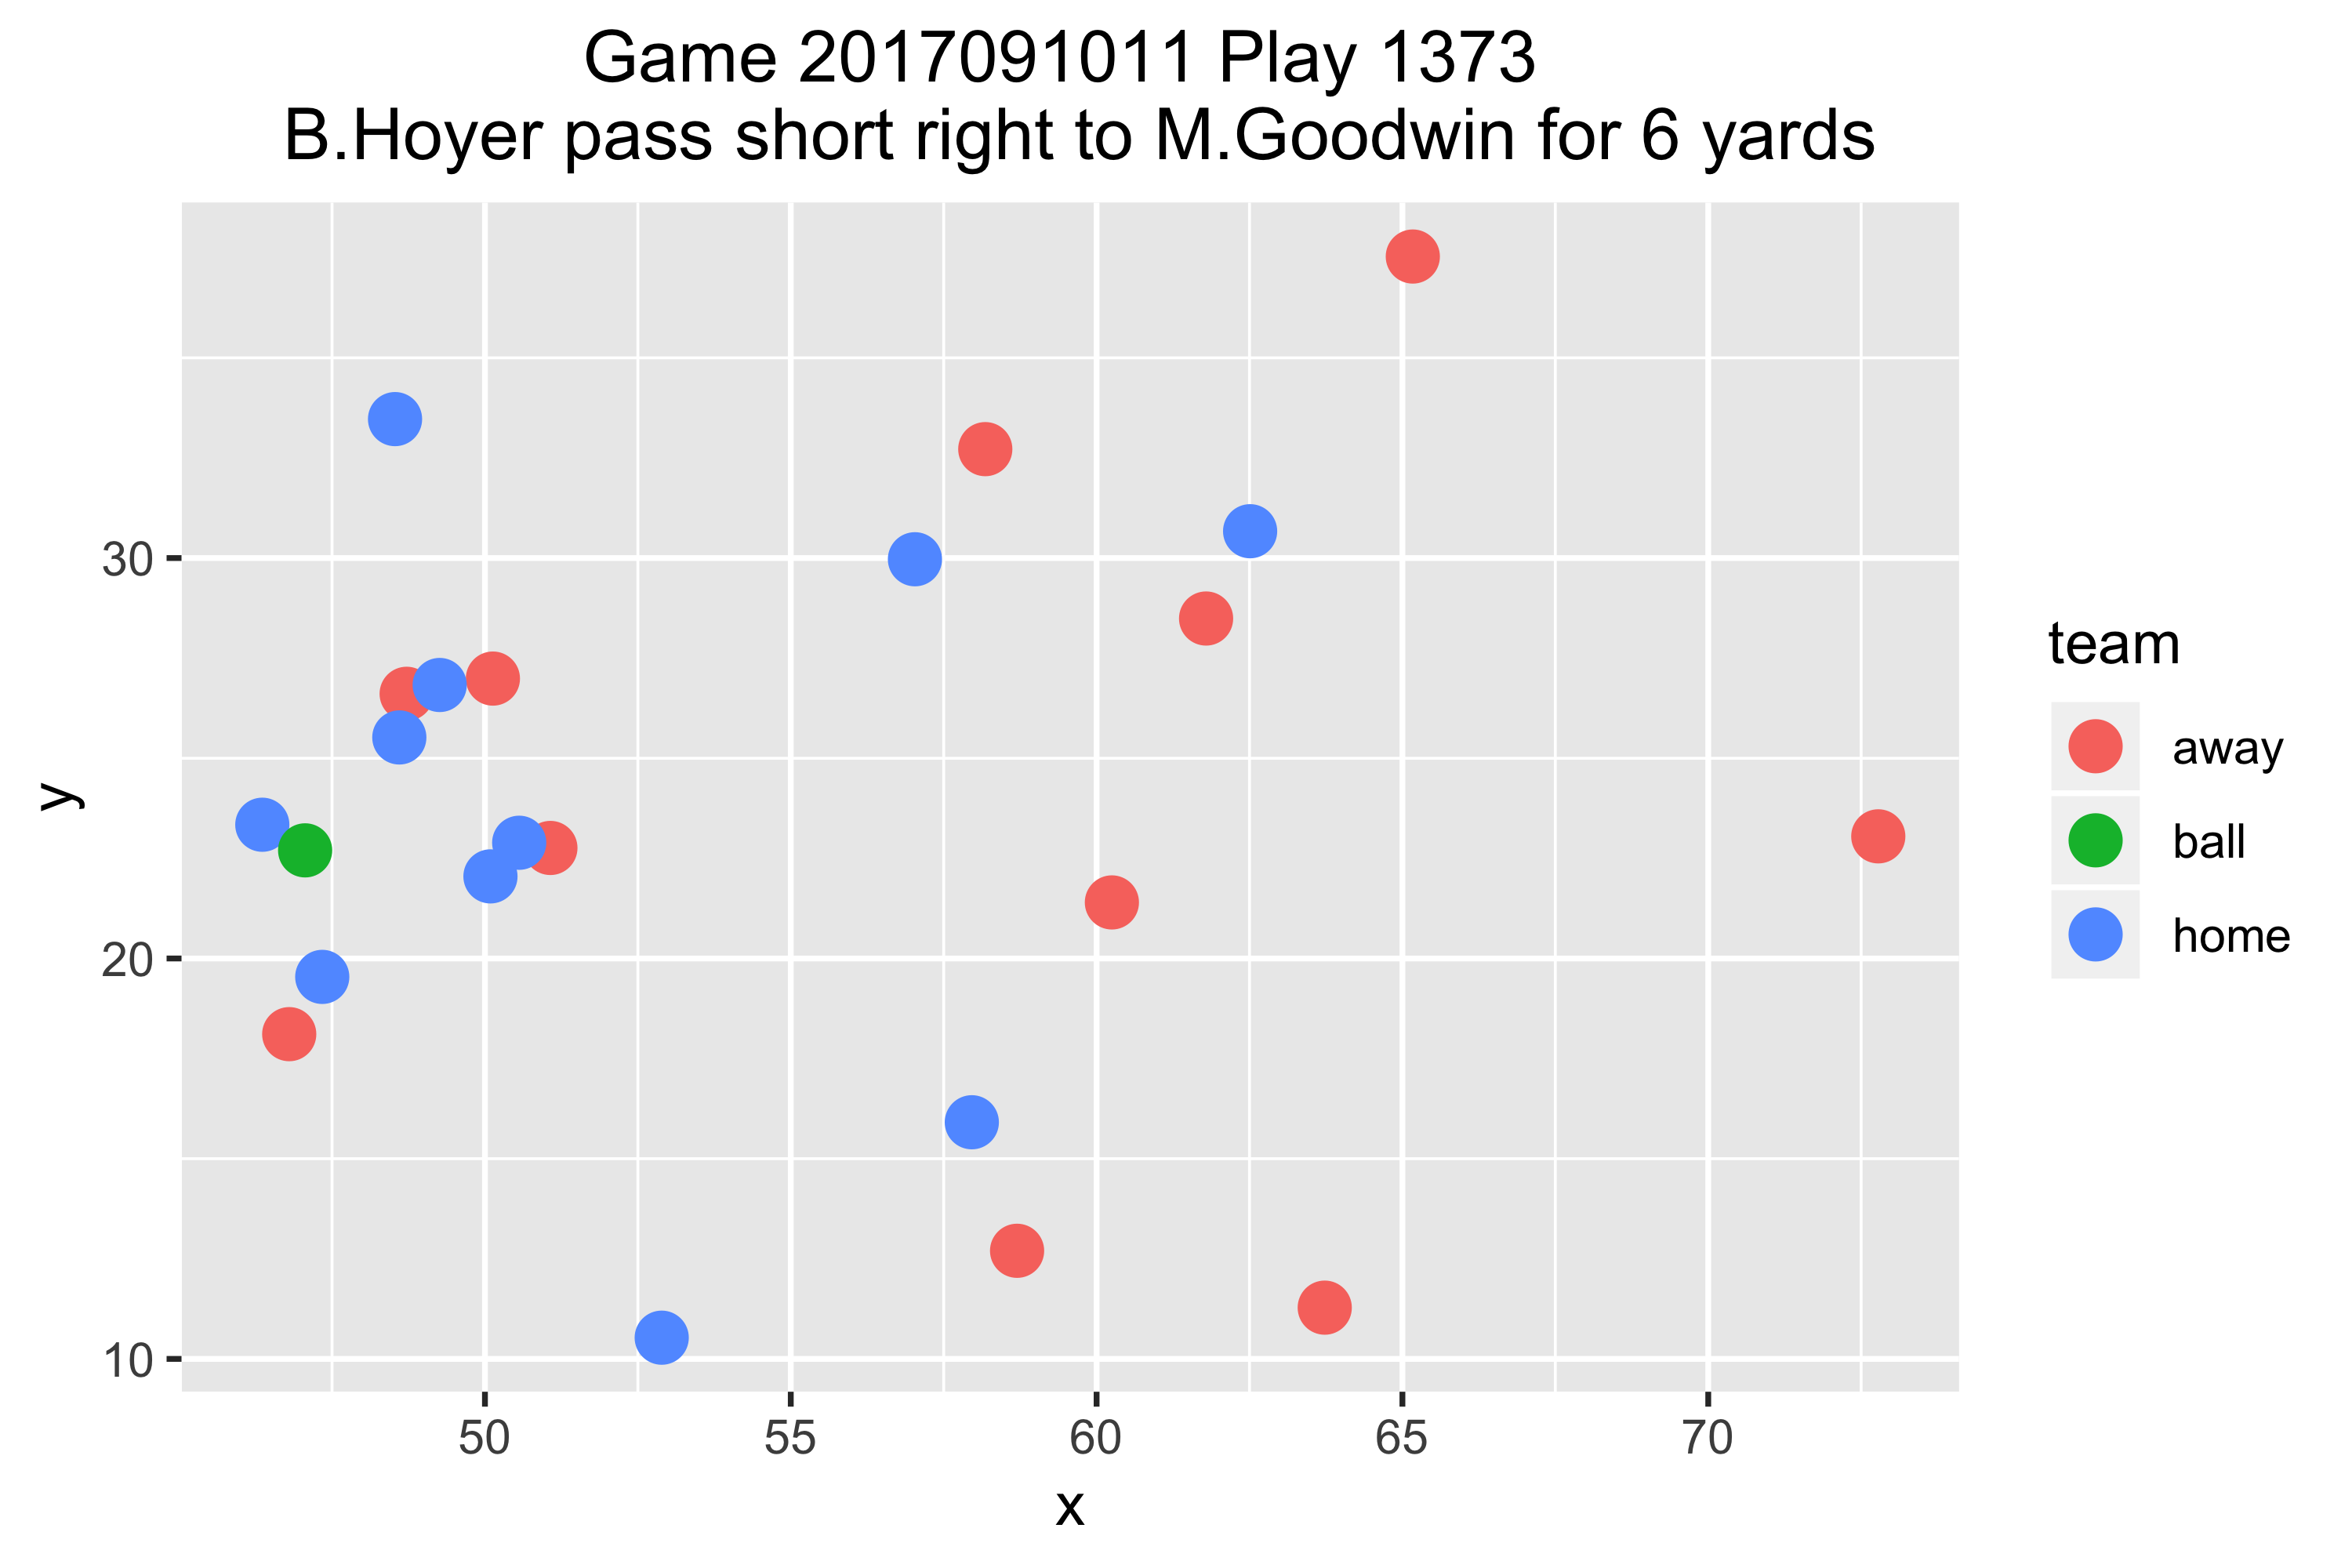
\includegraphics[width=0.8\textwidth]{good_separation.png}
\caption{A play with good separation between eligible receivers and closest defenders right before the ball is thrown.}
\end{figure}

\begin{figure}[h!]
\centering
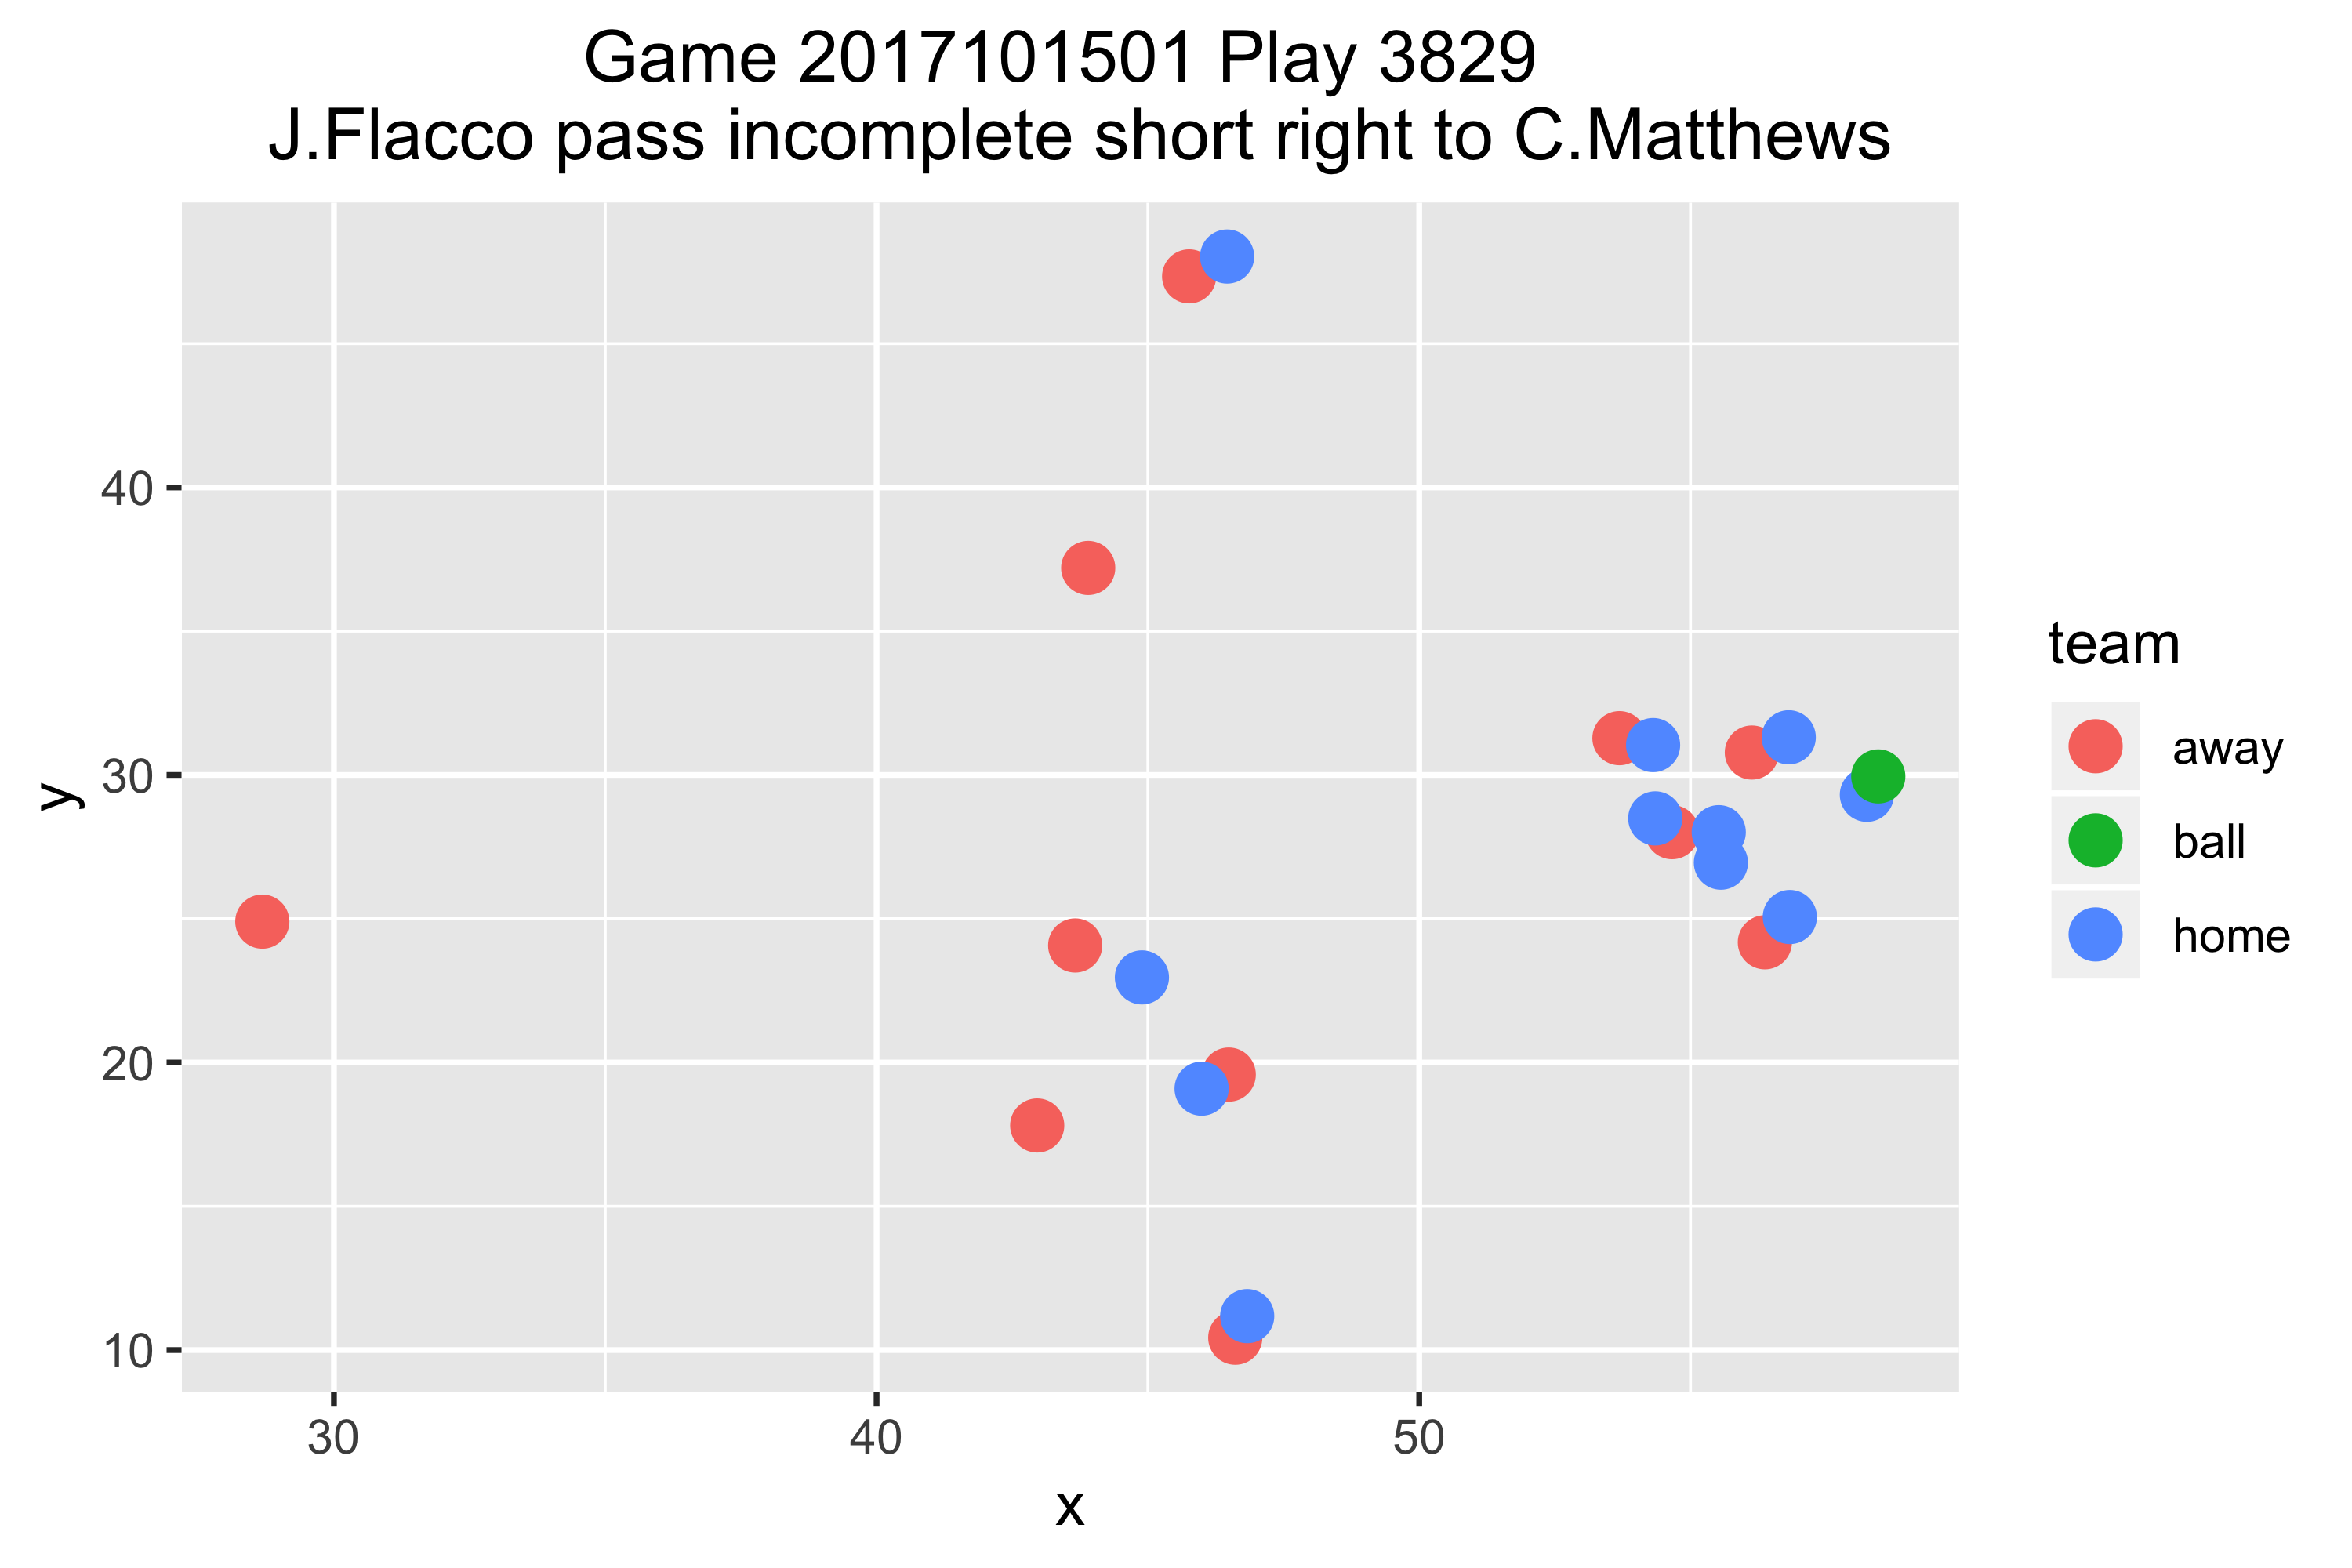
\includegraphics[width=0.8\textwidth]{bad_separation.png}
\caption{A play with bad separation between eligible receivers and closest defenders right before the ball is thrown.}
\end{figure}

\newpage
\subsection*{Exploratory Analysis}
%Outline of calculation procedure/algorithm \& issues for the separation itself
 
We determined ``standard'' eligible receivers in a play by identifying non-quarterback players whose numbers were under 50 or greater than 79. Because plays in which offensive linemen and defensive players reported as eligible were inconsistently labeled in the data, we did not look at the paths of ``non-standard'' eligible personnel. Trick plays in which the QB was the receiver were not considered. Consequently, we obtained a vector of up to five non-zero distances between eligible receivers and their closest defender for each qualified third down passing play, as there are a maximum of five eligible receivers. 
%\begin{figure}[H]
%\centering
%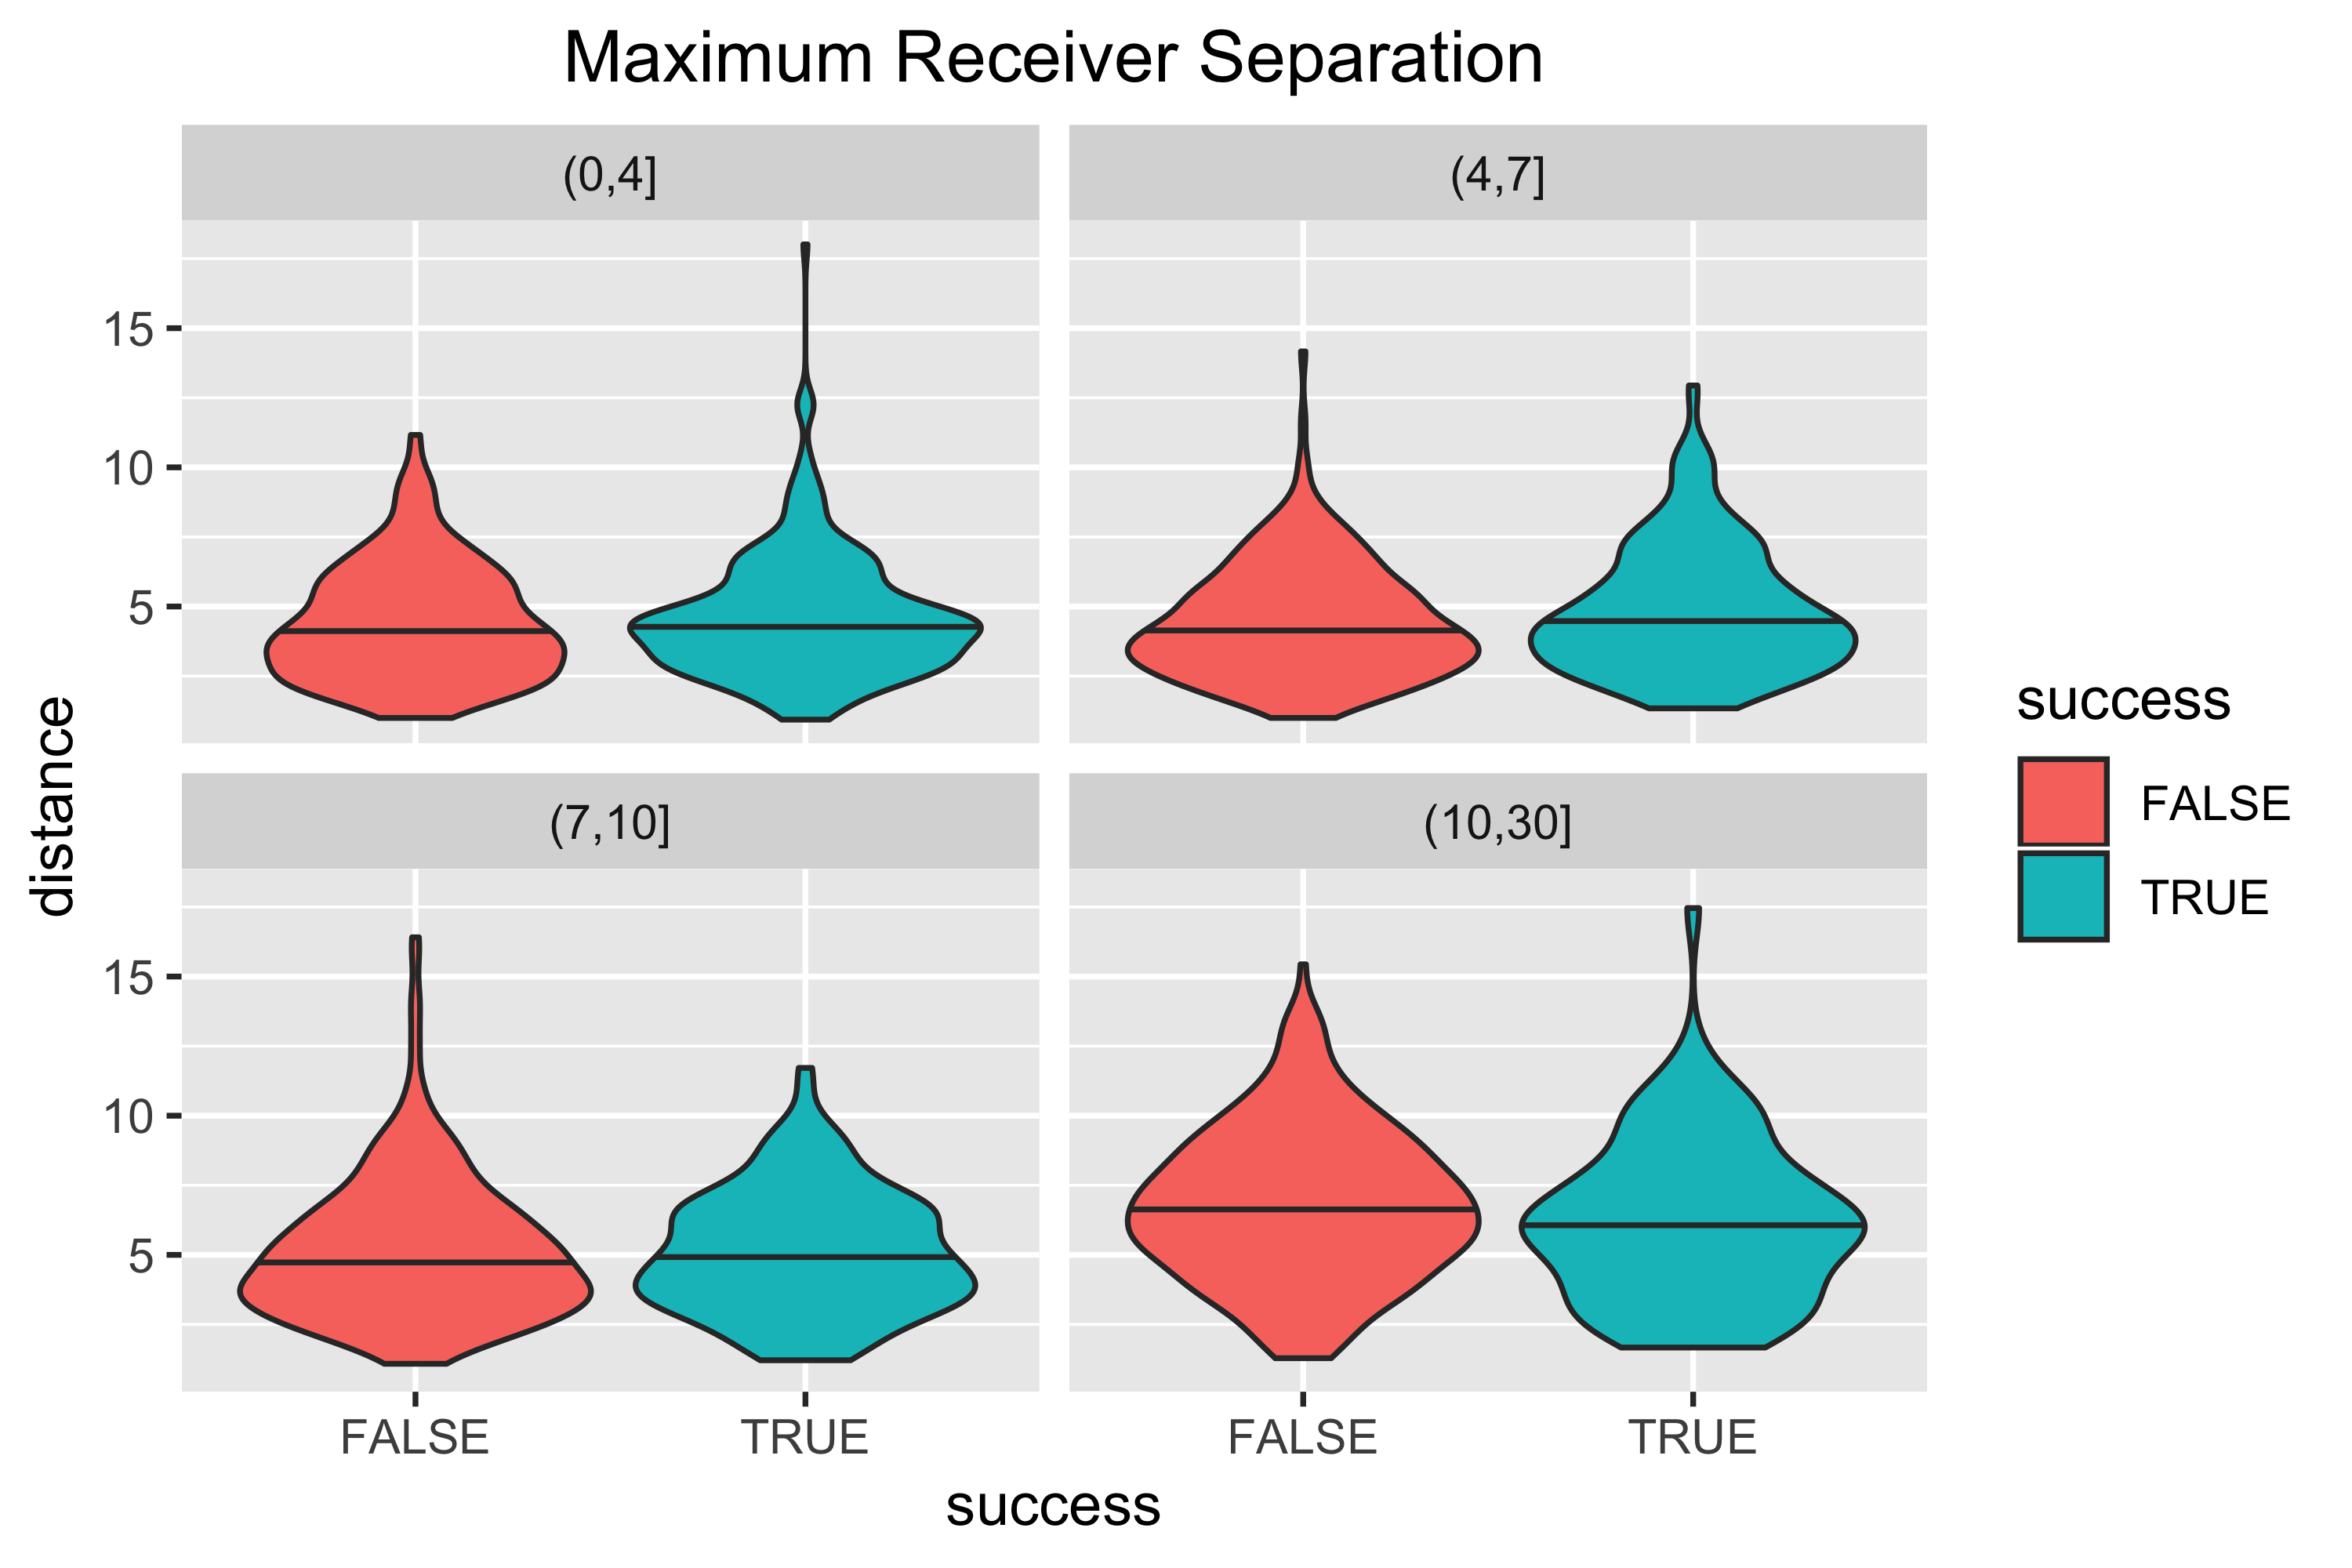
\includegraphics[width=0.8\textwidth]{max_separation.png}
%\caption{}
%\end{figure}

After iterating through all qualified third down passing plays, we plotted the means of minimum distance vectors corresponding to successes and failures in violin plots. Violin plots visualize the probability density of data, with y-axis displaying the range of possible data values, yards of separation in our case, and the thickness at the x-axis displaying how common that value of data appears in the sample.

The vectors and violin plots were additionally partitioned by ranges of yards-to-go until first down values. The ranges used for sorting were between 0 and 4 yards, between 4 and 7 yards, between 7 and 10 yards, and between 10 and 30 yards. We chose these numbers, as they marked the quartiles of the yards-to-go distribution. The extent of yards-to-go influences the routes chosen by the offense and coverage scheme used by the defense, so we wanted to observe if there were clearer differences in separation between successful and failed plays in some yards to go ranges than others, which could be linked to choice of play-calling.

\textbf{We hypothesized originally that mean separation distance for successful plays would exceed that of failed plays at every yards-to-go range. From Figure \ref{fig:violin}, we see that this hypothesis is supported with the mean separation being modestly higher in the successful case, approximately 0.19 yards higher in the 0 to 4 yards group, and approximately 0.22 yards higher in the 4 to 7 yards group.} For the 7 to 10 yard group, separation is higher by a hair's breadth. Curiously, in the 10 to 30 yard group, the failed case exhibits higher mean separation. A reason for this could be that defenses cover offenses more loosely in third and long situations that favor a bend-don't-break approach to prevent long passes. 

\begin{figure}[h!]
\centering
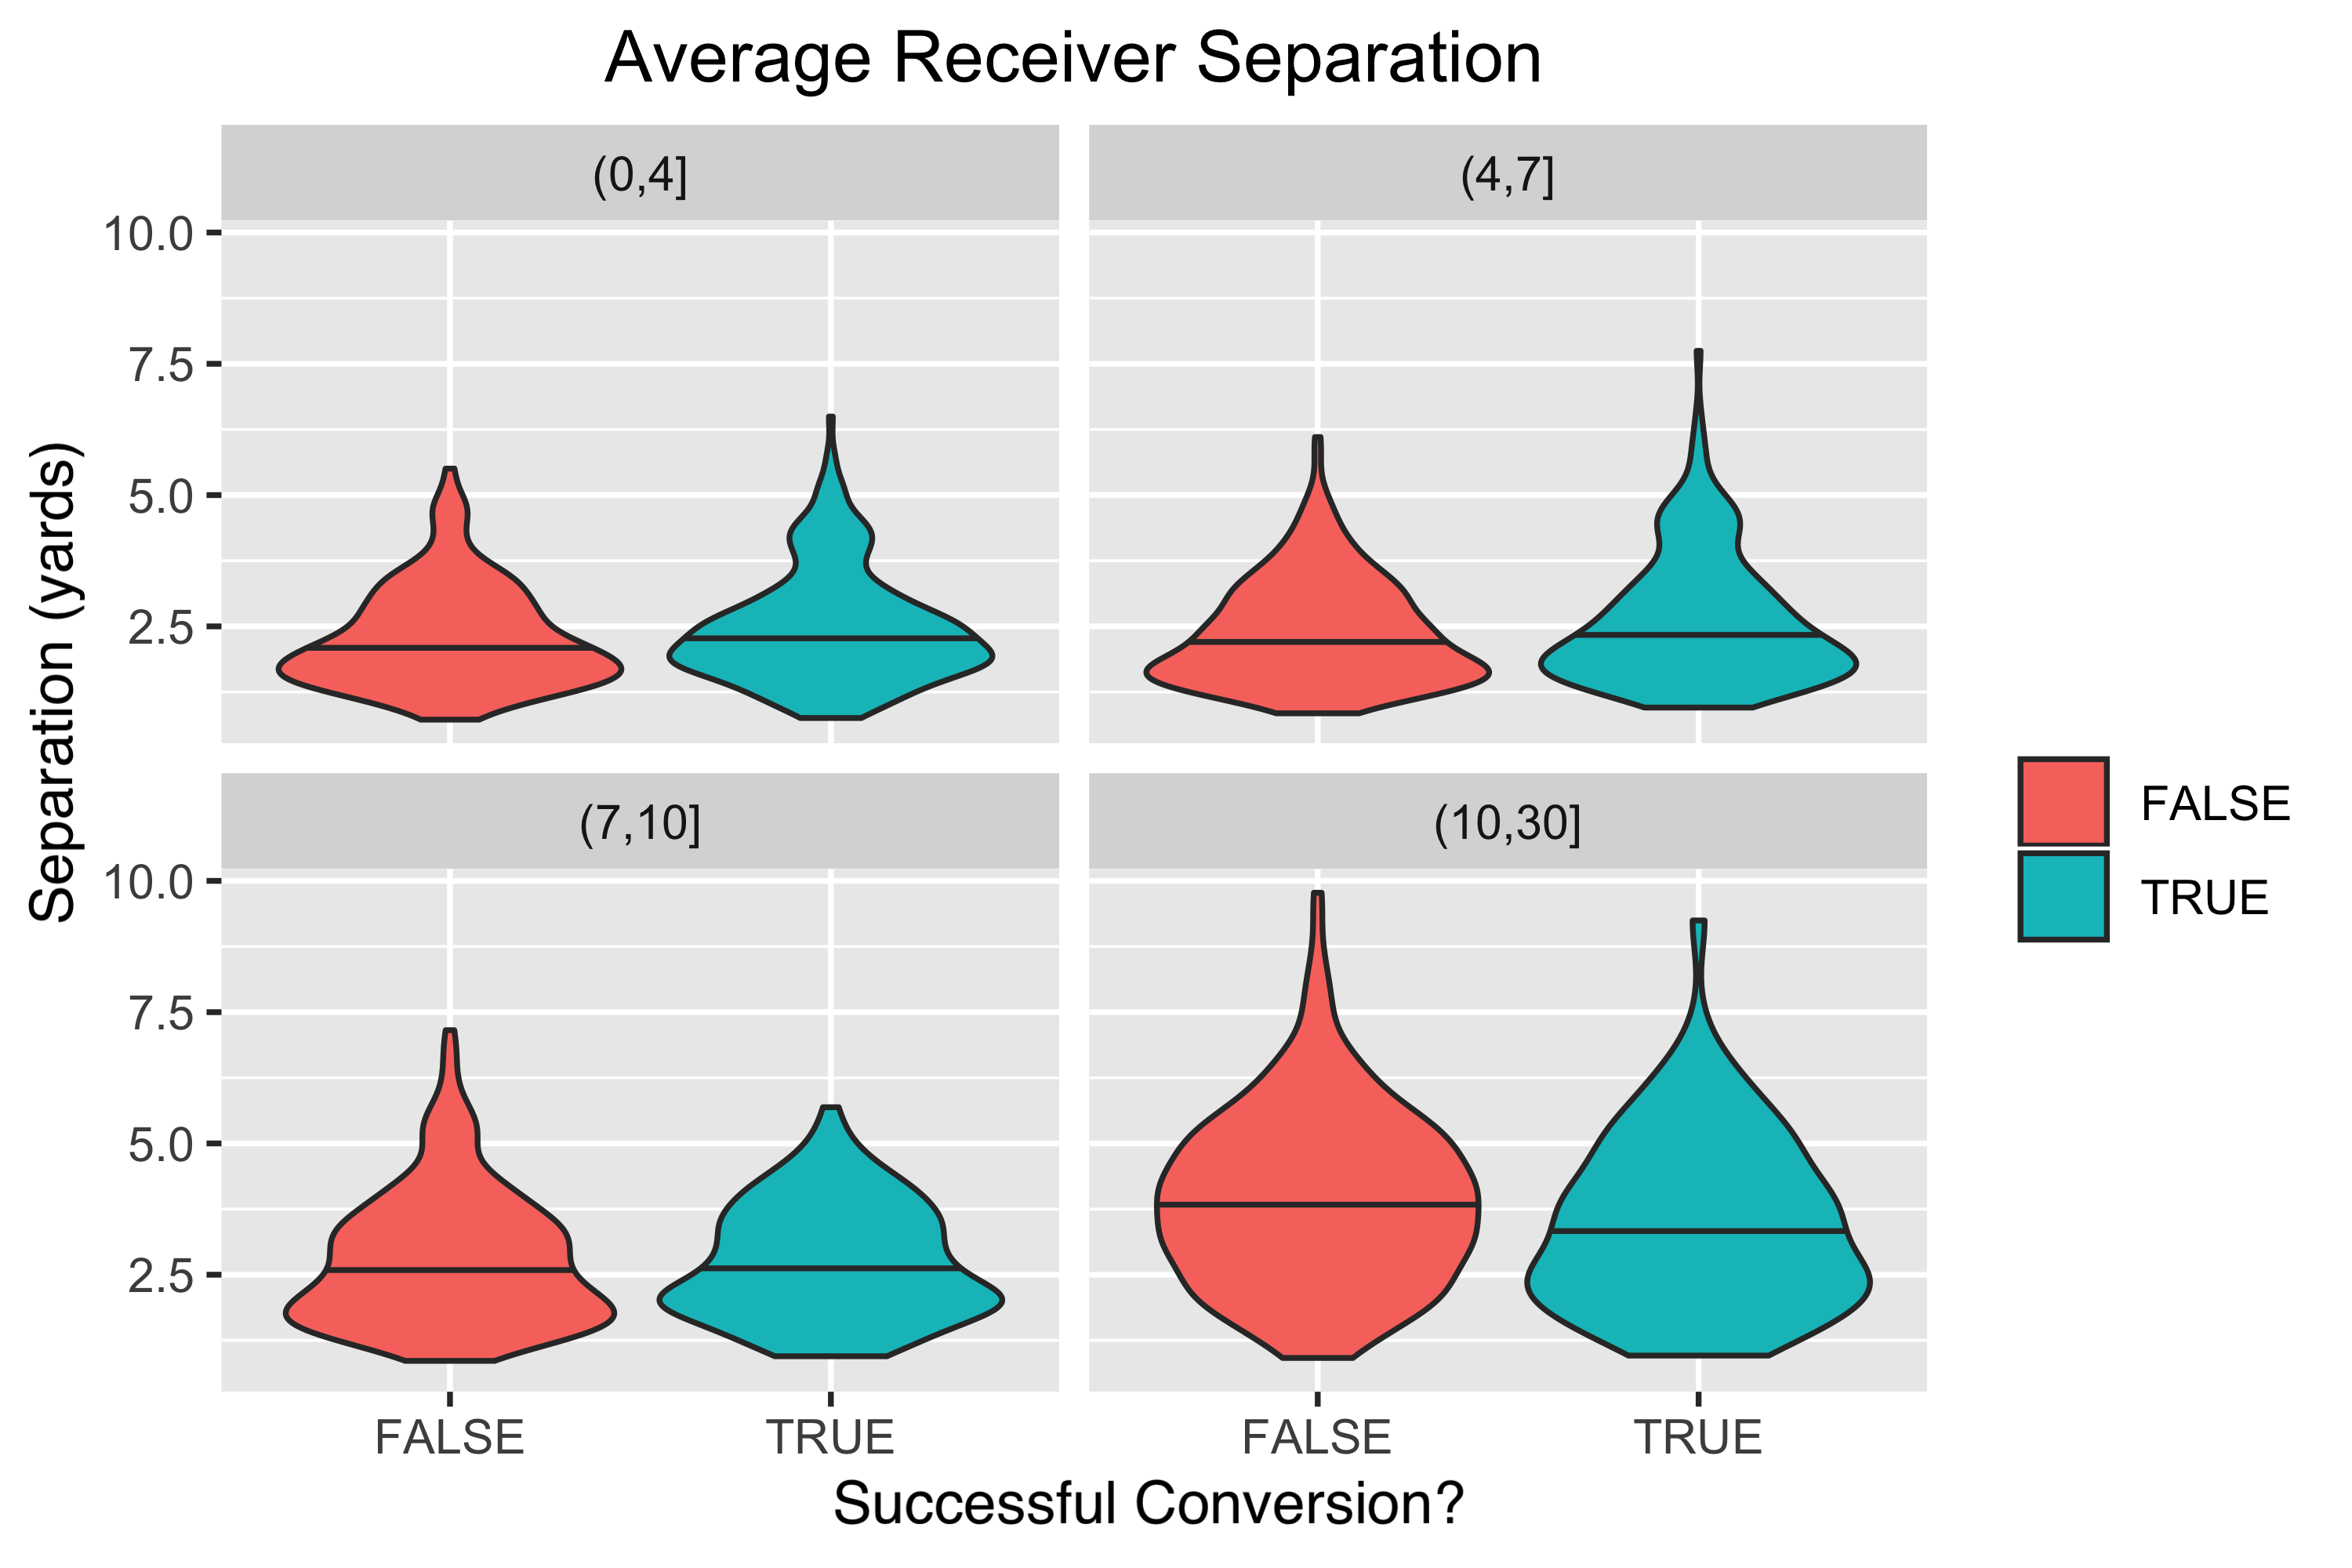
\includegraphics[width=0.8\textwidth]{mean_separation.png}
\caption{Distribution of average receiver separation for successful and failed plays grouped by yards to go.}
\label{fig:violin}
\end{figure}

\subsection*{Quantifying the Effect of Separation on Third Down Conversion with Logistic Models}

Figure \textbf{\ref{fig:violin}} suggests that separation and yards-to-go influence third down outcome, but are they significant factors? To look into this, we used a logistic regression model to estimate the size of the effect of separation and yards-to-go on conversion success. The logistic regression model is a standard tool for analyzing binary outcomes in many fields of research including medicine and artificial intelligence. Within each yards-to-go group, the model will calculate the odds as a function of separation.

The model results show a statistically significant correlation between separation and success adjusting for yards-to-go; in the model, the regression coefficient for separation has p-value 0.0435. \textbf{We observe that when there are less than 7 yards to go, the odds are estimated to increase with more separation. In particular, the probability of a successful attempt is estimated to shift from approximately 49\% to more than 62\% as the separation changes from 1 to 4 yards.} 

\begin{figure}[h!]
\centering
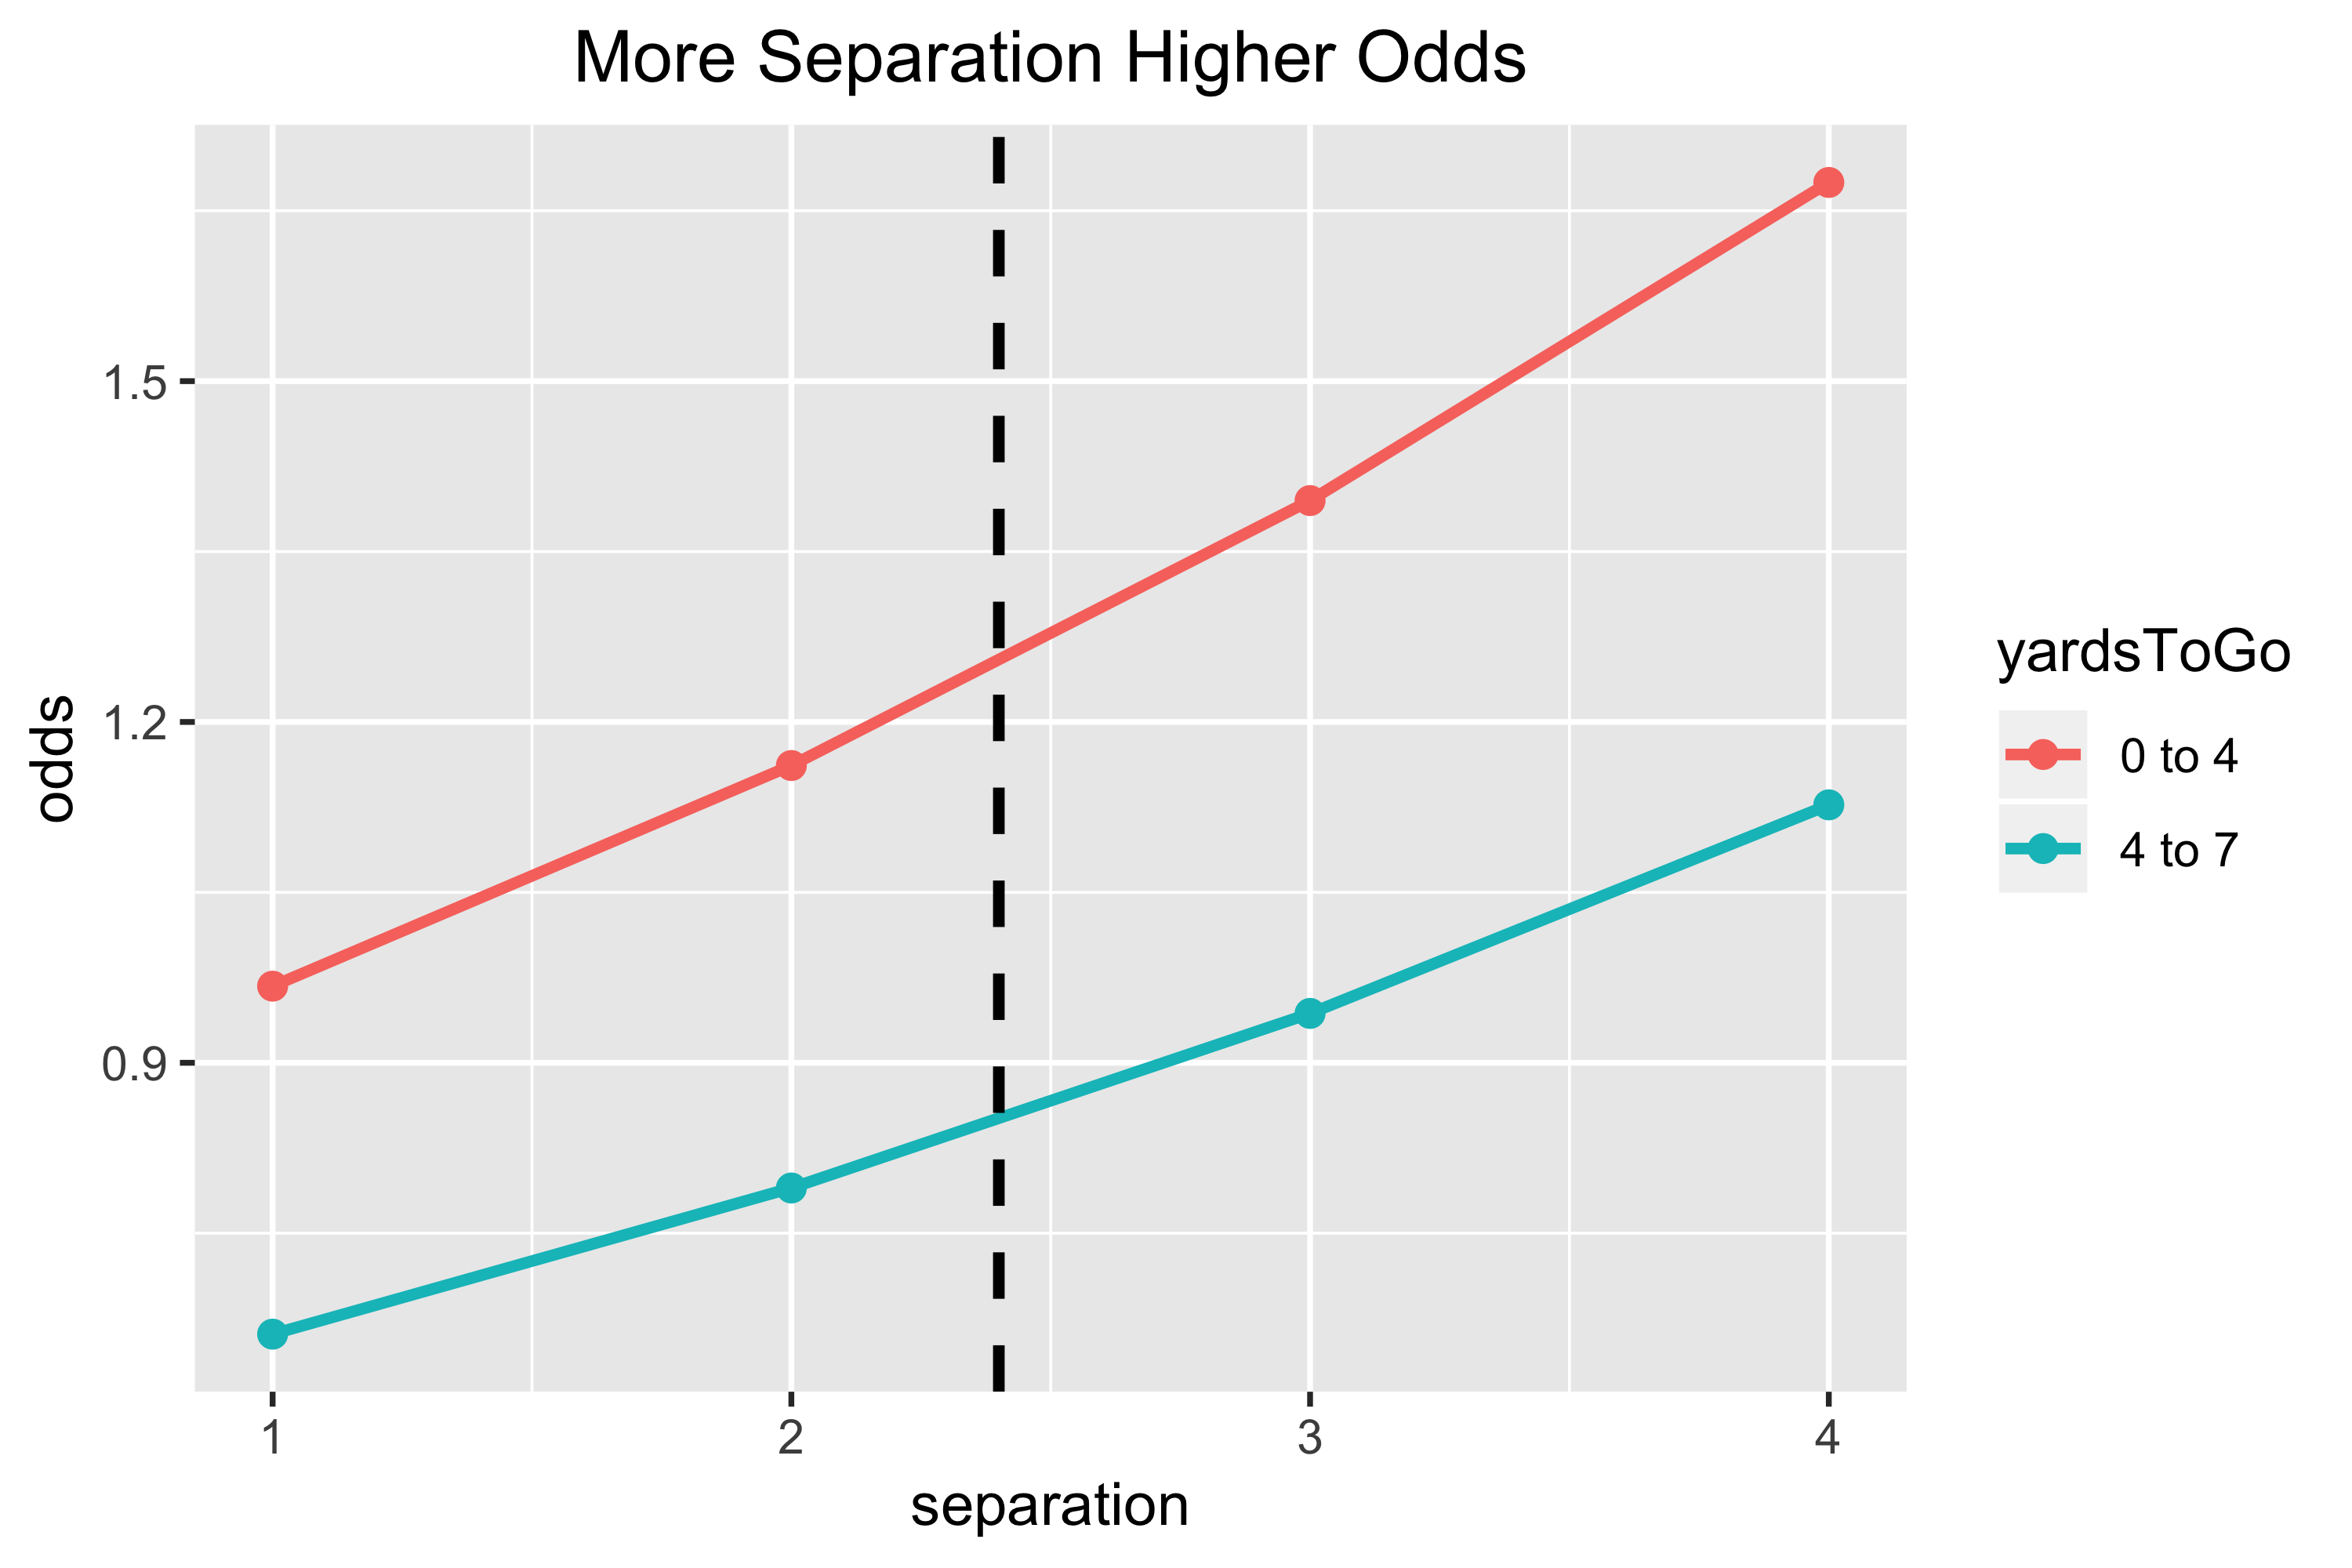
\includegraphics[width=0.8\textwidth]{odds_separation.png}
\caption{Expected odds for separation at different yards.}
\end{figure}

Note that the odds are calculated as the probability of success over the probability of failure. When the odds are 1, the probabilities of success and failure are both 50\%.

\section*{Analyzing The Influence of Route Type on Third Down Pass Outcome}

\subsection*{Route Identification}

\begin{figure}[h!]
\centering
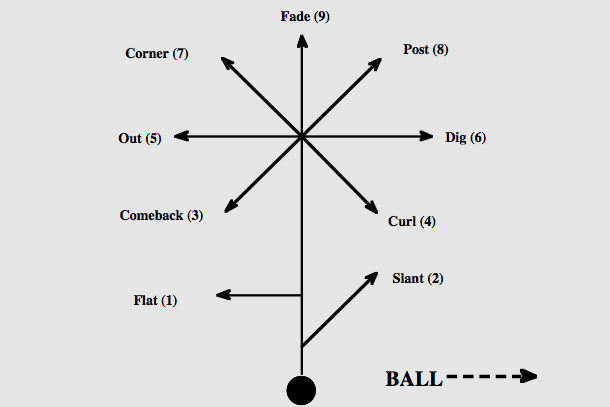
\includegraphics[width=0.8\textwidth]{routeTree.png}
\caption{The basic single-move route tree. Credit: Matt Bowen for \textit{Bleacher Report.}}
\label{fig:routeTree}
\end{figure}
%\section*{Logistic Regression Models on Third Down Pass Plays}

Building on our previous analysis, we then observed the effect of the presence of the basic ``initial'' route types pictured in Figure \ref{fig:routeTree} in a play on third down conversions. To determine route type, we looked at the frames of each play ranging from the snap to pass arrival. We noted eligible receiver motion angles relative to the line of scrimmage immediately following the snap to identify slants and flats. Then, we flagged periods in receiver paths in which there were large relative changes in angles as ``moves.'' The route was classified into route type based in the angle of the first move relative to the line of scrimmage, hence the use of the word ``initial'' above.

Of course, there are more complicated routes corresponding to multiple specific receiver moves and changes in direction, such as smash routes and sluggos. However, even classification of simple routes can be a noisy process, as routes can be expected to deviate from their ideal geometry. We did not want to limit route sample sizes by sorting into too many different route types. Thus, we kept to a simpler classification based on initial move angle.

\subsection*{Logistic Regression Model}

Following our preliminary classification of route types for third down passing plays, we built a logistic regression model to predict success with basic route type information. Having identified the basic routes, for each play, we created a count vector where each element is the total number of a particular route used in that play. This vector contained information about basic route types in the play. Along with the counts of basic routes, the model also took yards to go into account as before. 

\begin{figure}[h!]
\centering
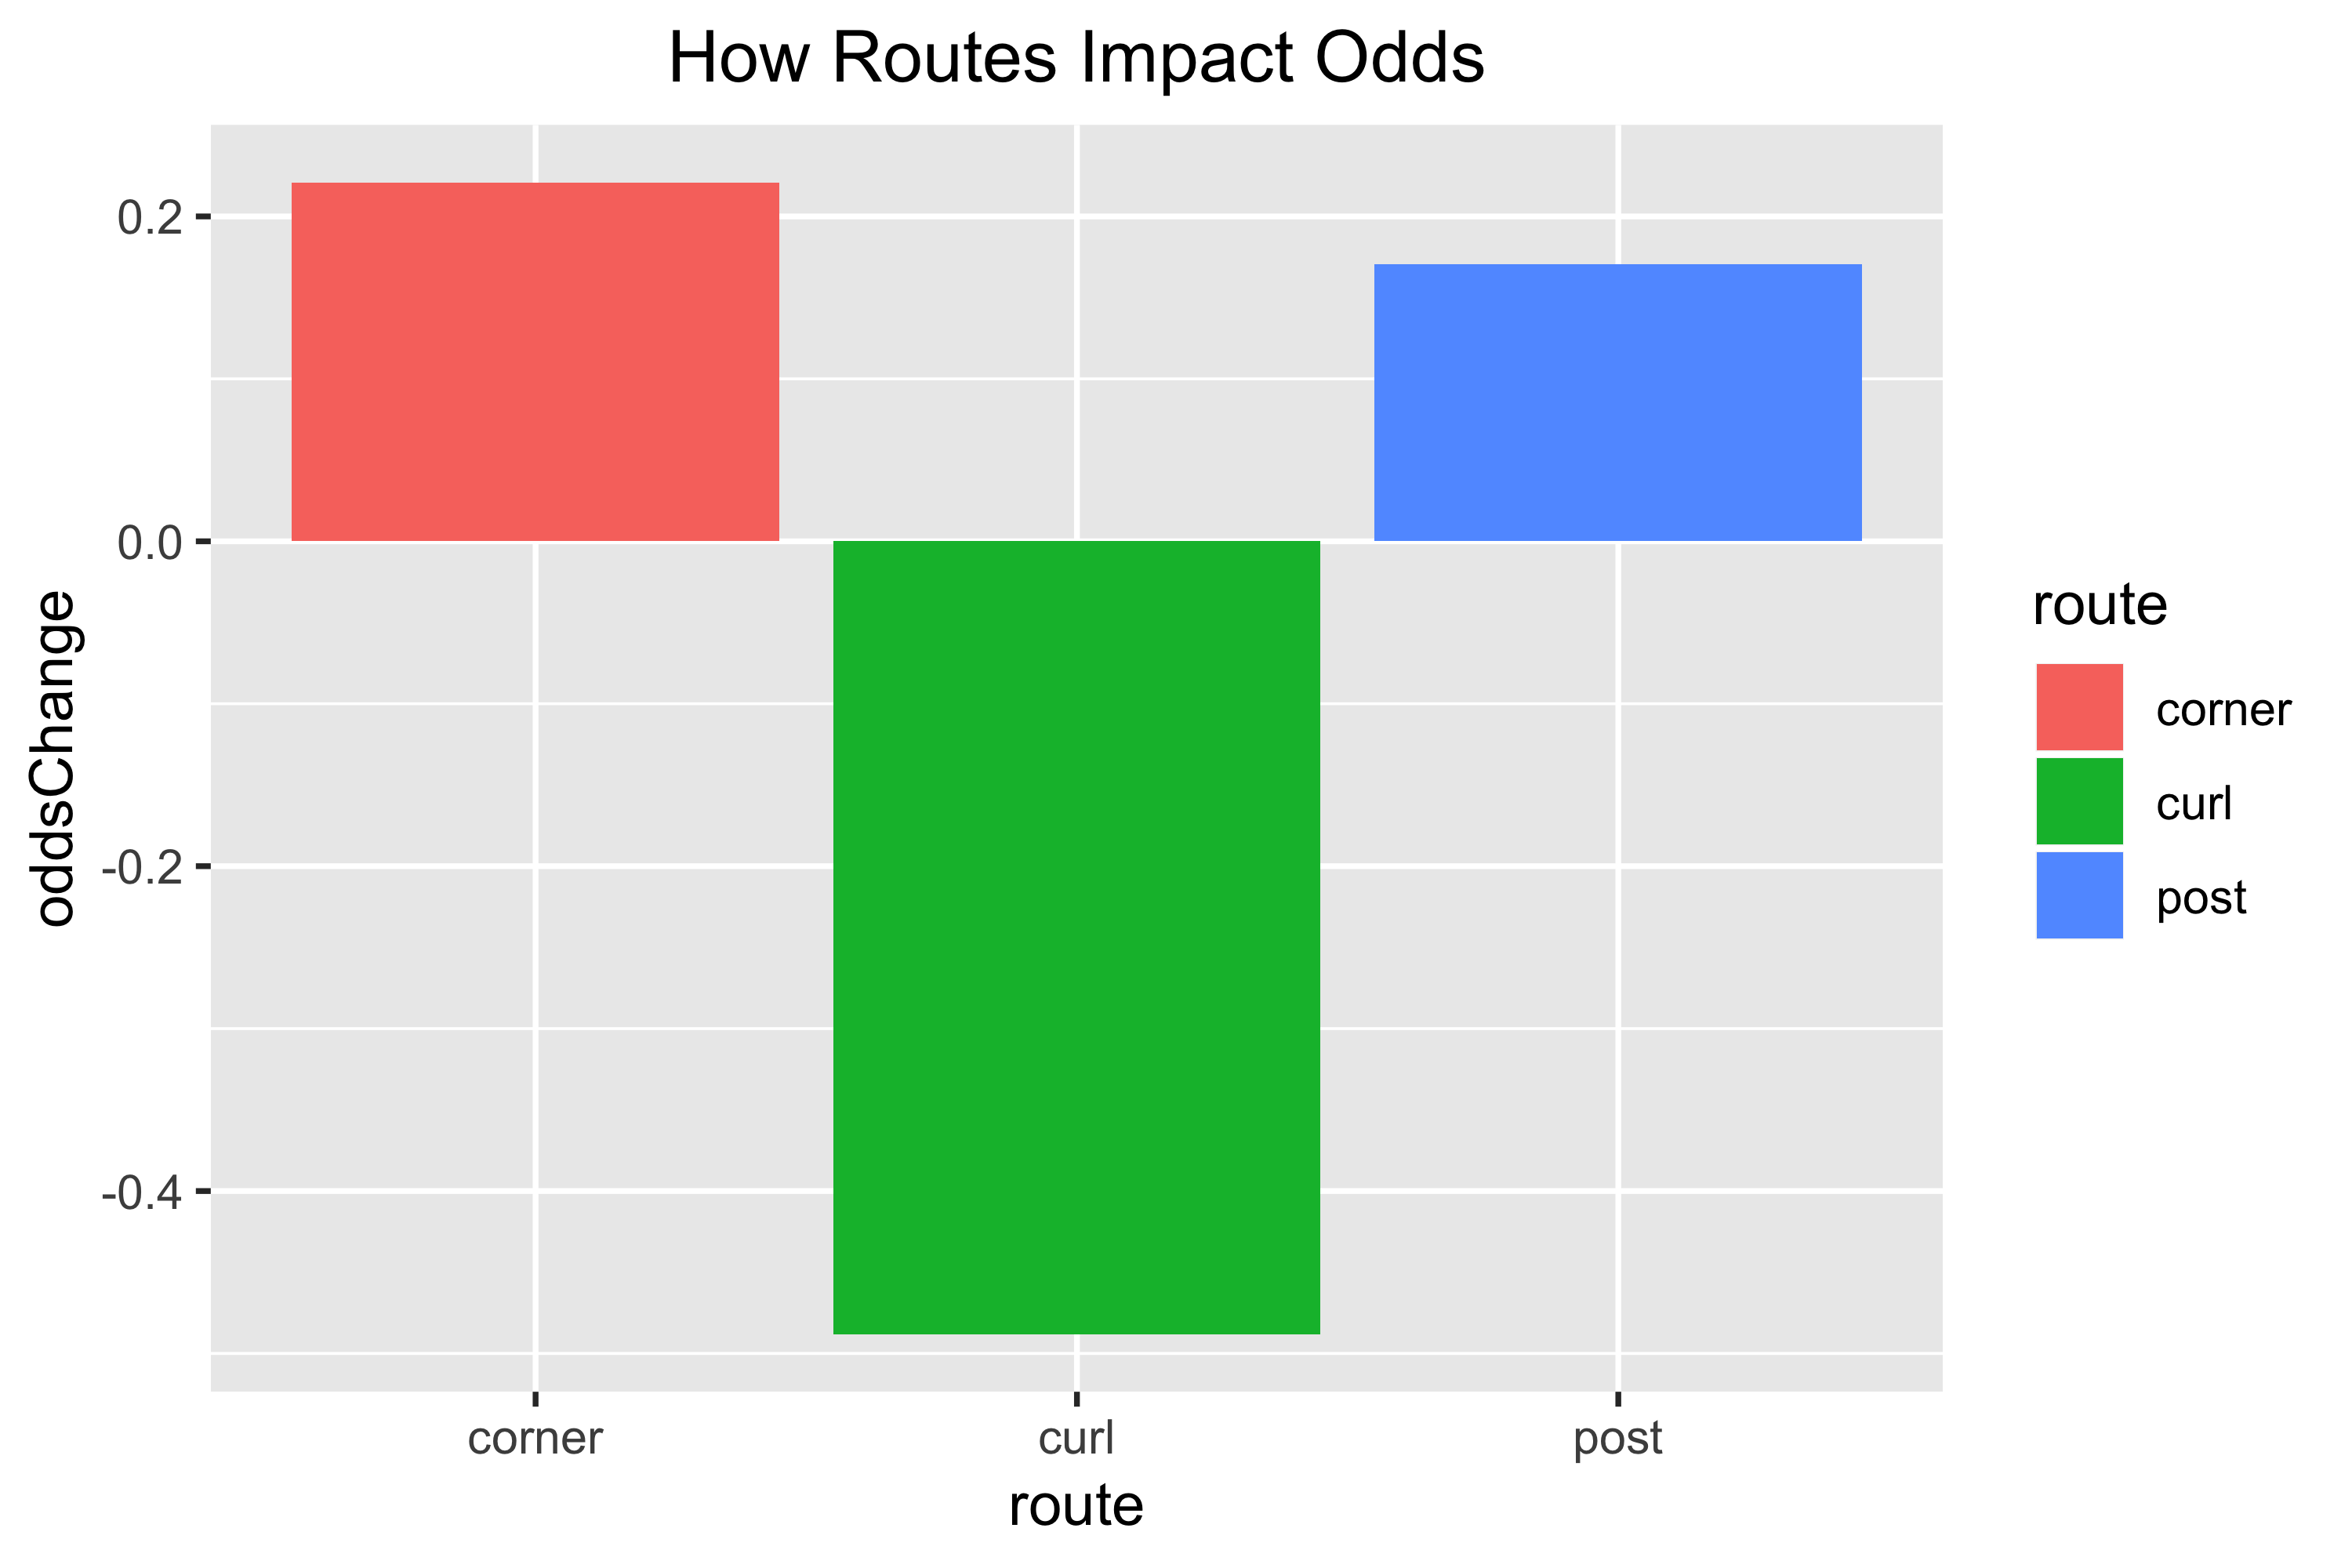
\includegraphics[width=0.8\textwidth]{odds_routes.png}
\caption{Change in expected odds when these basic route types are added to a play.}
\label{fig:route_odds}
\end{figure}

The results show that certain basic routes have statistically significant impacts on success adjusting for yards to go. \textbf{Given similar yards-to-go and the same other basic routes, the expected odds are estimated to be about 20\% higher when having an additional corner route, over 40\% lower when having an additional curl route, and almost 20\% higher when having an additional post route.} These significant impacts are illustrated in Figure \ref{fig:route_odds}.

While the model results are reasonable, there are several limitations. First, the basic route identification is not perfectly accurate but higher accuracy would likely improve the model. Second, the impacts of different routes are assumed to be additive as, for instance, the impact of corner combined with slant is the sum of the impact of corner and the impact of slant. However, it is possible that some routes when combined would lead to an extra impact beyond the sum. This can be modeled by interaction terms but the possibilities are too many for the data. Lastly, the model results must be interpreted with care as one would not expect plays with 5 corner routes to have 100\% higher odds.

\subsection*{Plays Demonstrating Model Results}

To illustrate the effect of routes at a qualitative level, we look at two particular plays. In Figure 7, Mitch Trubisky completes a deep corner pass for a successful third down conversion. In Figure 8, Tom Brady completes a pass to a curl route, but does not succeed in gaining the first down. These plays highlight the importance of route choice as shown in Figure 6 above. 


\begin{figure}[h!]
\centering
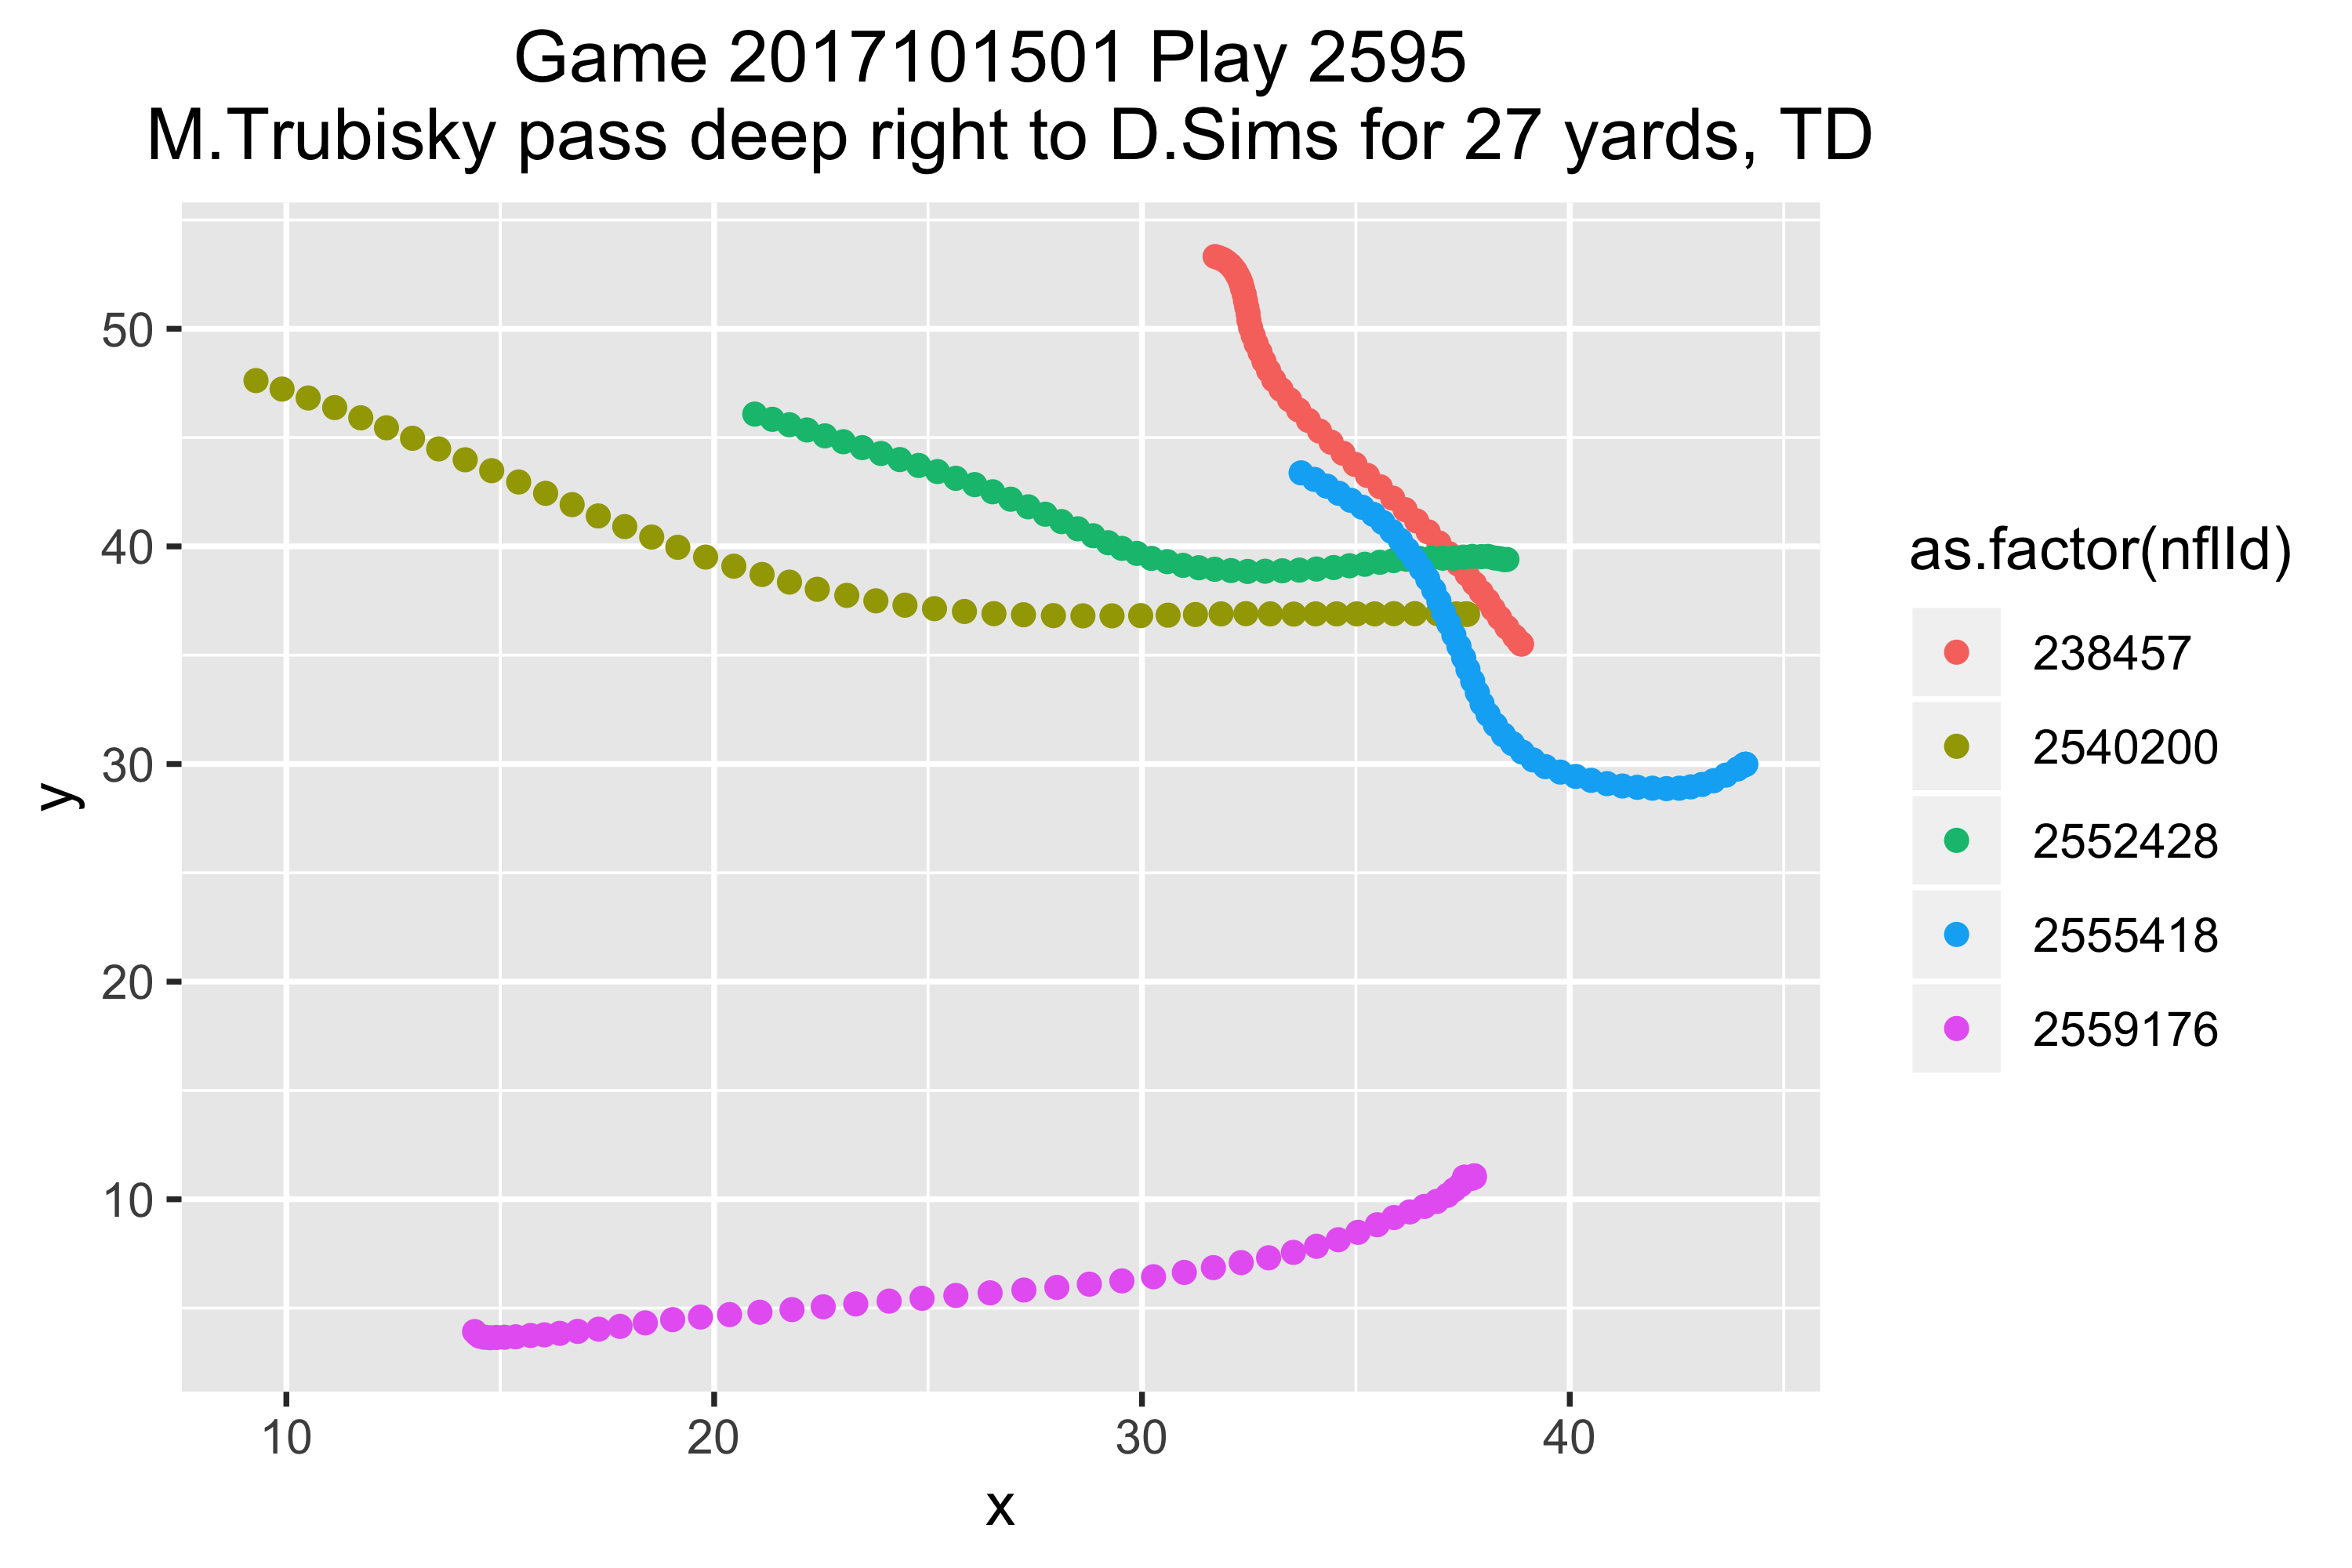
\includegraphics[width=0.8\textwidth]{good_post.png}
\caption{Successful Conversion}
\end{figure}


\begin{figure}[h!]
\centering
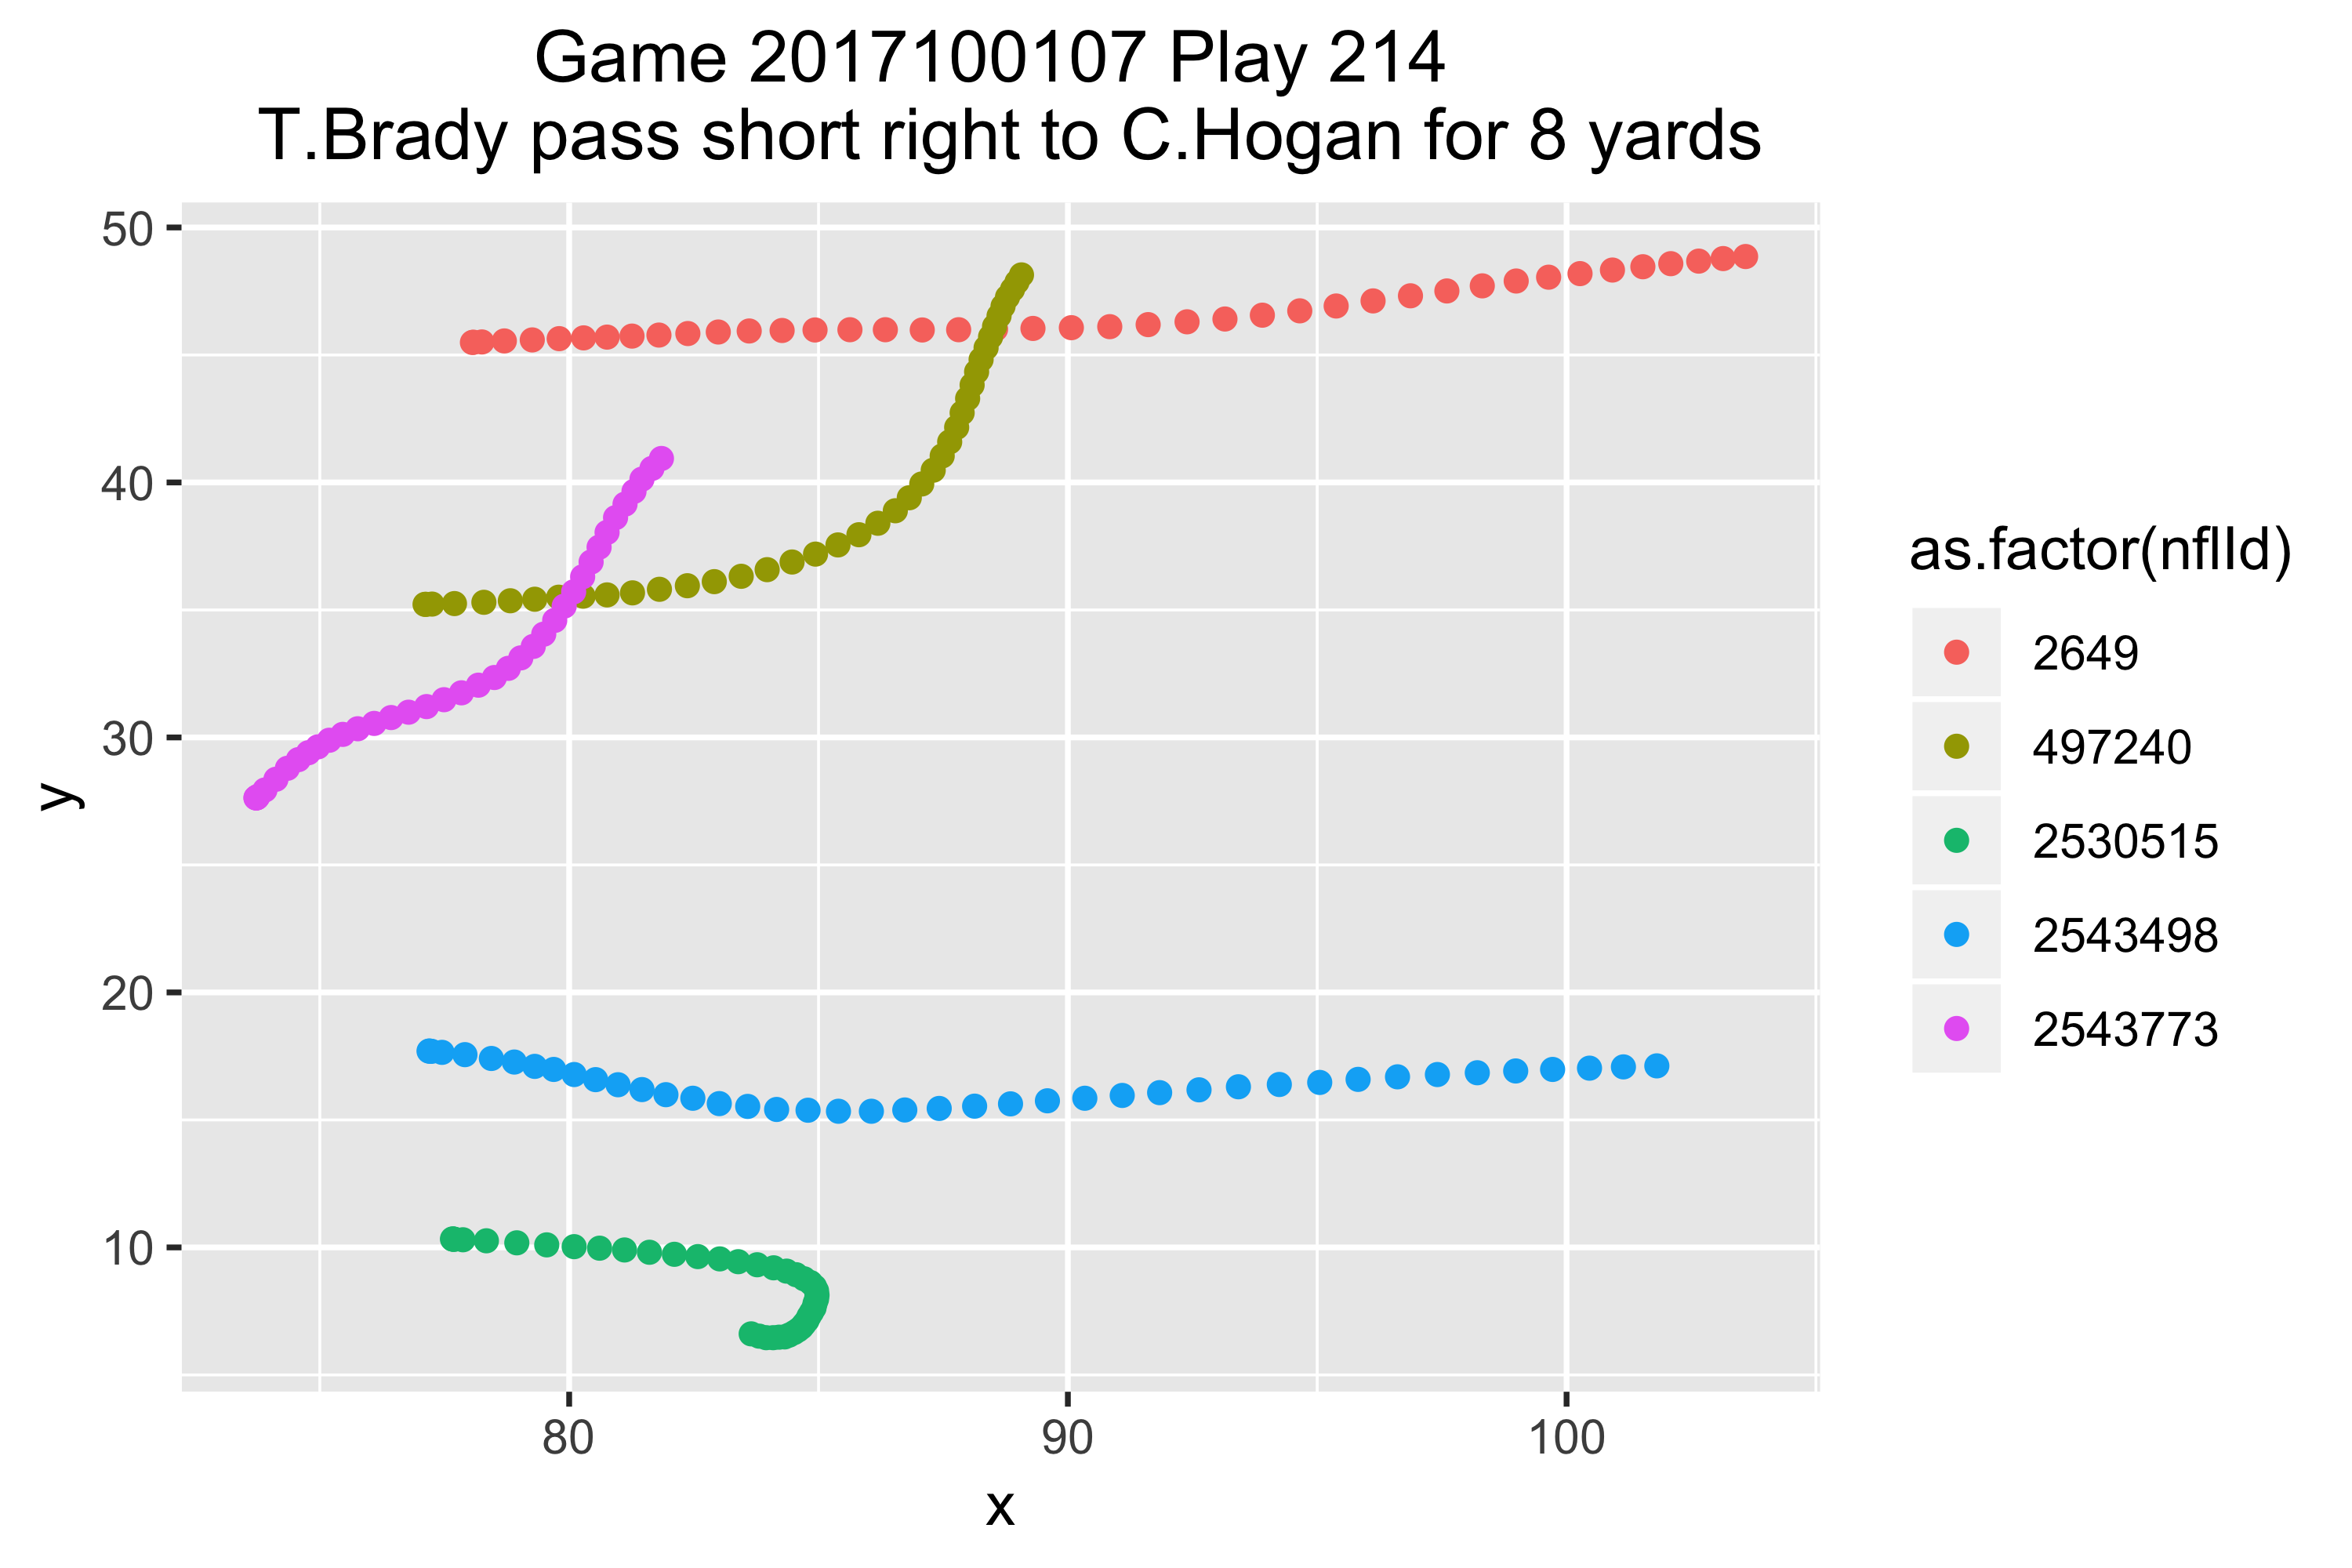
\includegraphics[width=0.8\textwidth]{bad_curl.png}
\caption{Failed Conversion}
\end{figure}

\subsection*{Analyzing The Effect of Route Type on Separation}

We tried to build a linear regression model for separation using the same variables above. However, the model failed to capture any correlation between basic route types and separation before the ball is thrown as indicated by low $r^2$ value in the model output (last in the Appendix). This is likely because this analysis attempted to connect the separation at the single frame when the quarterback made his decision, with the many frames that make up a route. In the future, we would want to use the separation data from all of the frames of each play to analyze the affect of routes on separation throughout the play. While the frame the ball is released shows what information was available to the quarterback at the time of his decision, it cannot describe anticipated separation. This is where we expect the additional temporal information to be useful. In particular, the change in separation between when the ball is thrown and arrives would capture the effects of anticipatory throwing.


\section*{Conclusion}
Third down conversions rates are arguably the most important statistic for NFL offenses. A conversion is the difference between keeping your drive alive or giving possession away with a punt. Repeated successful conversions can wear away at the opponents' mental states while boosting yours. In short, third down plays are crunch time, make or break moments that put both teams to the test. 

More than $70\%$ of third down plays (in the given data) are pass plays. As demonstrated above, \textbf{the level of separation is crucial in predetermining the success of a third down catch}. When yards to go are in the short to medium range (0-7 yards), this increase in odds is statistically significant (Figure 4). Moreover, the odds of converting your third-down attempt are dependent on the type of routes ran by the receivers. In particular, having an additional corner route in your route combination is expected to increase your odds of converting by more than $20\%$ (Figure 5).

Finally, with more time, we would have liked to look further into the maximum separation between each receiver and his defender at any point during the receiver's route (instead of just at the time of the throw). This easily leads into more analyses that consider full-route information instead of a single frame. Furthermore, a hypothesis worth exploring is that catch-rate increases as separation increases; less pressure, higher chances of making a catch. Additionally, with more game data, we can examine factors leading to higher separation for individual teams vs. our aggregated results. 

With the insights gained from our analysis, coaches and playmakers will be better equipped to call/run plays that fit their future third down scenarios. We have also laid a groundwork for future analyses that can take in richer information for routes and individual teams. Following these lines of research, teams can remain strong competitors for seasons to come.

\newpage

\section*{Appendix: Model Output}

\begin{lstlisting}[frame=single]
> summary(fit)

Call:
glm(formula = success ~ fly + out + comeback + curl + dig + slant + 
    corner + post + yardsToGo.levels, family = "binomial", data = play.data.combo)

Deviance Residuals: 
    Min       1Q   Median       3Q      Max  
-1.9218  -1.0562  -0.6001   0.9901   1.8529  

Coefficients:
                         Estimate Std. Error z value Pr(>|z|)    
(Intercept)              0.609845   0.182455   3.342  0.00083 ***
fly                      0.032460   0.103601   0.313  0.75404    
out                     -0.002358   0.145139  -0.016  0.98704    
comeback                -0.088292   0.194088  -0.455  0.64917    
curl                    -0.669634   0.238408  -2.809  0.00497 ** 
dig                     -0.039464   0.079548  -0.496  0.61982    
slant                   -0.027330   0.056747  -0.482  0.63008    
corner                   0.199605   0.071027   2.810  0.00495 ** 
post                     0.157602   0.073416   2.147  0.03182 *  
yardsToGo.levels(4,7]   -0.373032   0.155434  -2.400  0.01640 *  
yardsToGo.levels(7,10]  -1.160025   0.163423  -7.098 1.26e-12 ***
yardsToGo.levels(10,30] -1.847458   0.177586 -10.403  < 2e-16 ***
---
Signif. codes:  0 ‘***’ 0.001 ‘**’ 0.01 ‘*’ 0.05 ‘.’ 0.1 ‘ ’ 1

(Dispersion parameter for binomial family taken to be 1)

    Null deviance: 1859.0  on 1340  degrees of freedom
Residual deviance: 1701.4  on 1329  degrees of freedom
AIC: 1725.4

Number of Fisher Scoring iterations: 4

\end{lstlisting}

\begin{lstlisting}[frame=single]
> summary(fit)

Call:
glm(formula = success ~ fly + out + comeback + curl + dig + slant + corner + post + yardsToGo.levels, 
    family = "binomial", 
    data = play.data.combo)

Deviance Residuals: 
    Min       1Q   Median       3Q      Max  
-1.9218  -1.0562  -0.6001   0.9901   1.8529  

Coefficients:
                         Estimate Std. Error z value Pr(>|z|)    
(Intercept)              0.609845   0.182455   3.342  0.00083 ***
fly                      0.032460   0.103601   0.313  0.75404    
out                     -0.002358   0.145139  -0.016  0.98704    
comeback                -0.088292   0.194088  -0.455  0.64917    
curl                    -0.669634   0.238408  -2.809  0.00497 ** 
dig                     -0.039464   0.079548  -0.496  0.61982    
slant                   -0.027330   0.056747  -0.482  0.63008    
corner                   0.199605   0.071027   2.810  0.00495 ** 
post                     0.157602   0.073416   2.147  0.03182 *  
yardsToGo.levels(4,7]   -0.373032   0.155434  -2.400  0.01640 *  
yardsToGo.levels(7,10]  -1.160025   0.163423  -7.098 1.26e-12 ***
yardsToGo.levels(10,30] -1.847458   0.177586 -10.403  < 2e-16 ***
---
Signif. codes:  0 ‘***’ 0.001 ‘**’ 0.01 ‘*’ 0.05 ‘.’ 0.1 ‘ ’ 1

(Dispersion parameter for binomial family taken to be 1)

    Null deviance: 1859.0  on 1340  degrees of freedom
Residual deviance: 1701.4  on 1329  degrees of freedom
AIC: 1725.4

Number of Fisher Scoring iterations: 4
\end{lstlisting}

\begin{lstlisting}[frame=single]
> summary(fit)

Call:
lm(formula = distance ~ fly + out + comeback + curl + dig + slant + 
    corner + post + yardsToGo.levels, data = play.data.combo)

Residuals:
    Min      1Q  Median      3Q     Max 
-3.0924 -0.9078 -0.1539  0.7514  5.6677 

Coefficients:
                        Estimate Std. Error t value Pr(>|t|)    
(Intercept)              2.83844    0.10802  26.278  < 2e-16 ***
fly                      0.02482    0.06098   0.407 0.684087    
out                      0.03631    0.08545   0.425 0.670951    
comeback                -0.02905    0.11318  -0.257 0.797445    
curl                     0.24054    0.13461   1.787 0.074173 .  
dig                     -0.02828    0.04698  -0.602 0.547234    
slant                   -0.18479    0.03368  -5.487 4.89e-08 ***
corner                  -0.07016    0.04169  -1.683 0.092666 .  
post                    -0.01641    0.04286  -0.383 0.701892    
yardsToGo.levels(4,7]    0.10927    0.09337   1.170 0.242099    
yardsToGo.levels(7,10]   0.36256    0.09748   3.719 0.000208 ***
yardsToGo.levels(10,30]  1.45236    0.09907  14.661  < 2e-16 ***
---
Signif. codes:  0 ‘***’ 0.001 ‘**’ 0.01 ‘*’ 0.05 ‘.’ 0.1 ‘ ’ 1

Residual standard error: 1.256 on 1329 degrees of freedom
Multiple R-squared:  0.1937,	Adjusted R-squared:  0.187 
F-statistic: 29.02 on 11 and 1329 DF,  p-value: < 2.2e-16
\end{lstlisting}


\end{document}